\documentclass{article}

\usepackage[spanish]{babel}
\usepackage[utf8]{inputenc}

\usepackage{graphicx}
\graphicspath{{./../imgs/}}

\usepackage{geometry}
\geometry{a4paper, margin=1in}

\title{Laboratorio 1: Proyecto LEDs}
\author{Gonzalo G. Fernández}
\date{\today}

\begin{document}
\maketitle

\section*{Descripción}

El proyecto consiste en la implementación de la arquitectura de la Fig. \ref{fig:scheme} mediante el uso de Verilog.

\begin{figure}[ht]
    \centering
    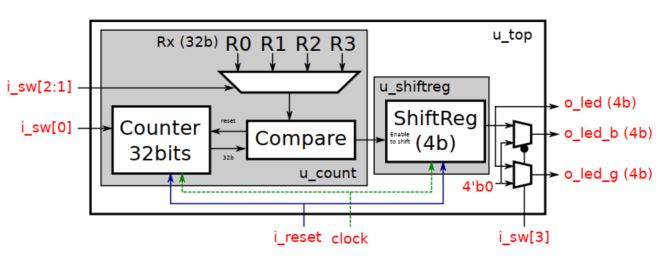
\includegraphics[]{./scheme.jpg}
    \caption{Esquema de diseño a implementar}
    \label{fig:scheme}
\end{figure}

Los nombres en rojo son puertos.
\begin{itemize}
    \item \textit{i\_reset} es el reset del sistema, el cual pone a cero el contador e inicializa el shift register (SR).
    \item \textit{i\_sw[0]} controla el enable (1) del contador. En estado (0) todo se detiene sin alterar el estado actual del contador y del SR.
    \item El SR se desplaza únicamente cuando el contador llegó a algún límite R0-R3.
    \item La elección del límite se puede realizar en cualquier momento del funcionamiento mediante \textit{i\_sw[2:1]}.
    \item \textit{i\_sw[3]} elige el color de los LEDs RGB.
\end{itemize}

\section*{Diseño en Verilog}

En la Fig. \ref{fig:rtl-schematic} se puede observar el esquemático resultante del análisis RTL del diseño realizado.

\begin{figure}[ht]
    \centering
    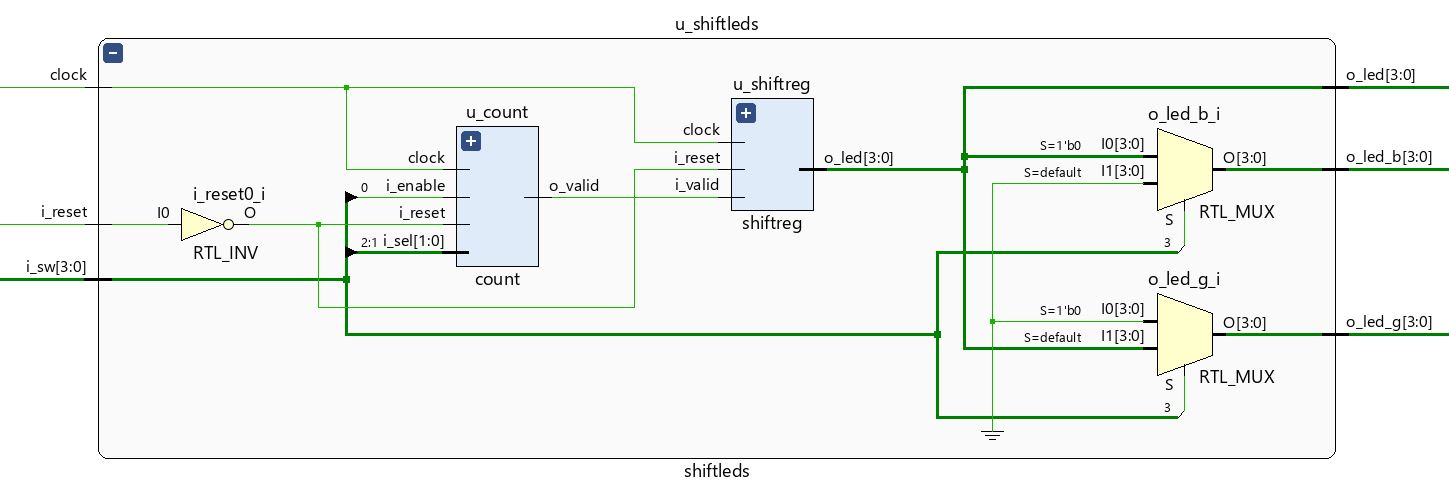
\includegraphics[width=\textwidth]{rtl_schematic.jpg}
    \caption{Esquemático de diseño a partir de análisis RTL}
    \label{fig:rtl-schematic}
\end{figure}

\section*{Simulación de comportamiento}

En la Fig. \ref{fig:behavioral-sim} se puede observar las formas de ondas resultantes de una simulación de comportamiento producida mediante el testbench diseñado.

\begin{figure}[ht]
    \centering
    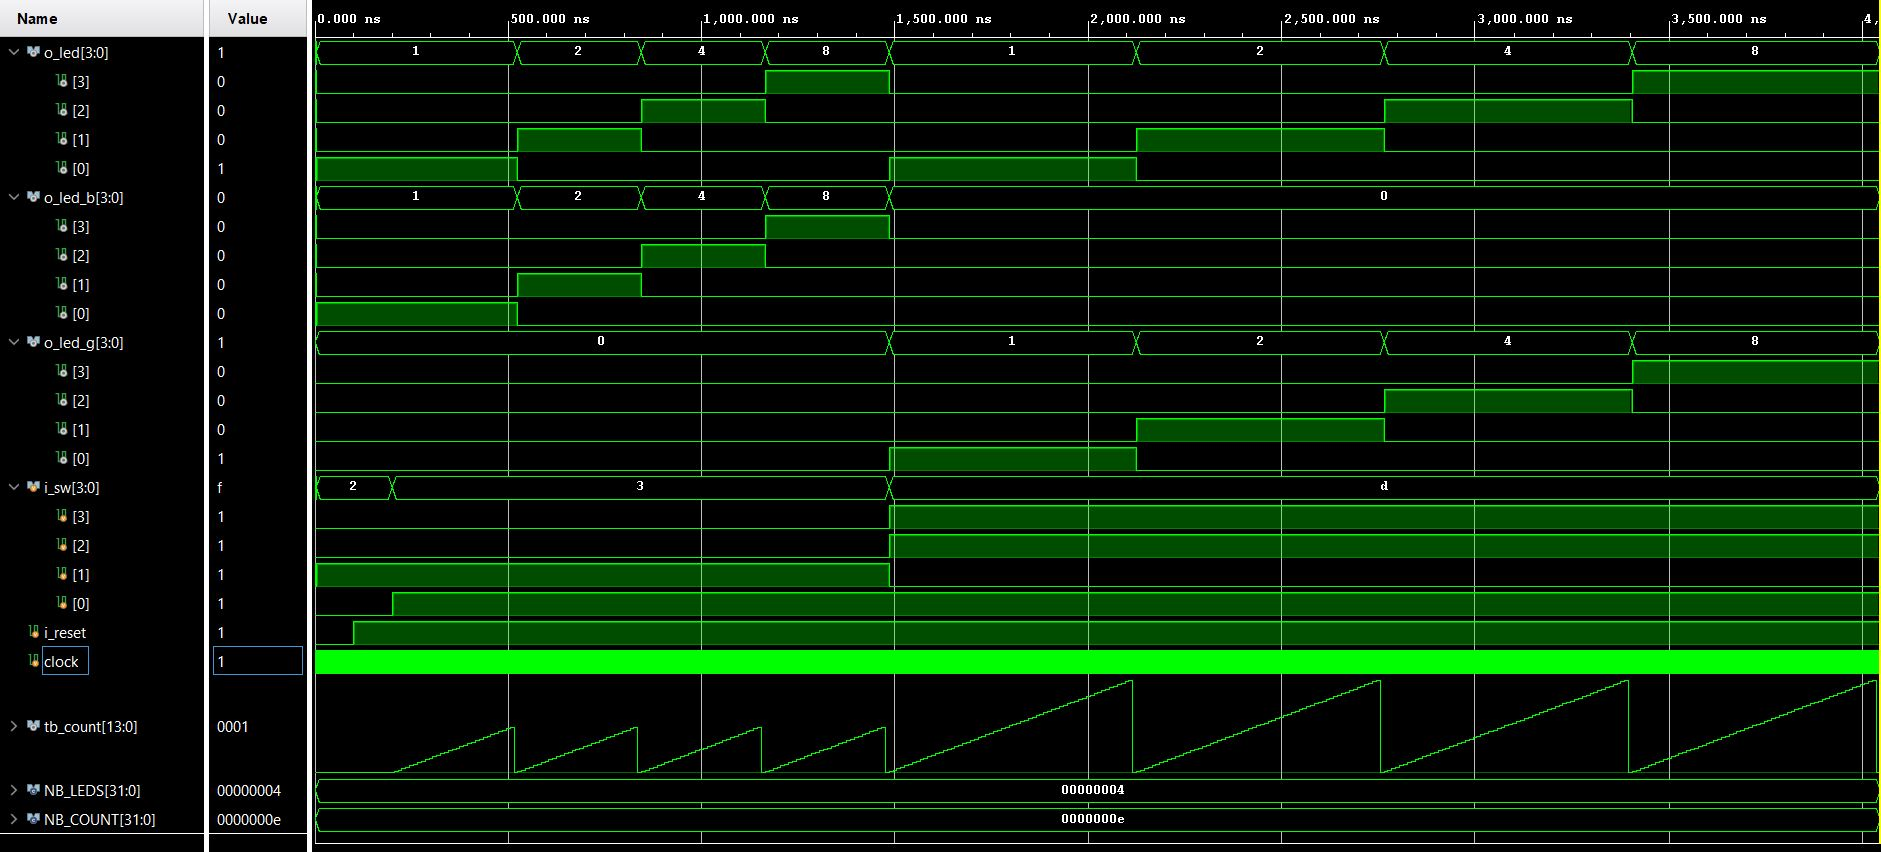
\includegraphics[width=\textwidth]{behavioral_sim.jpg}
    \caption{Forma de onda obtenida mediante simulación de comportamiento}
    \label{fig:behavioral-sim}
\end{figure}

\section*{Implementación: Módulos VIO e ILA}

Se implementan los IP cores Virtual Input/Output (VIO) e Integrated Logic Analyzer (ILA) para utilizarlos como interfaz y trabajar con el servidor remoto de FPGAs.

En la Fig. \ref{fig:ila-waveform} se observa la forma de onda obtenida con ILA ante un trigger al leer un 4 en el estado de los LEDs.

\begin{figure}[ht]
    \centering
    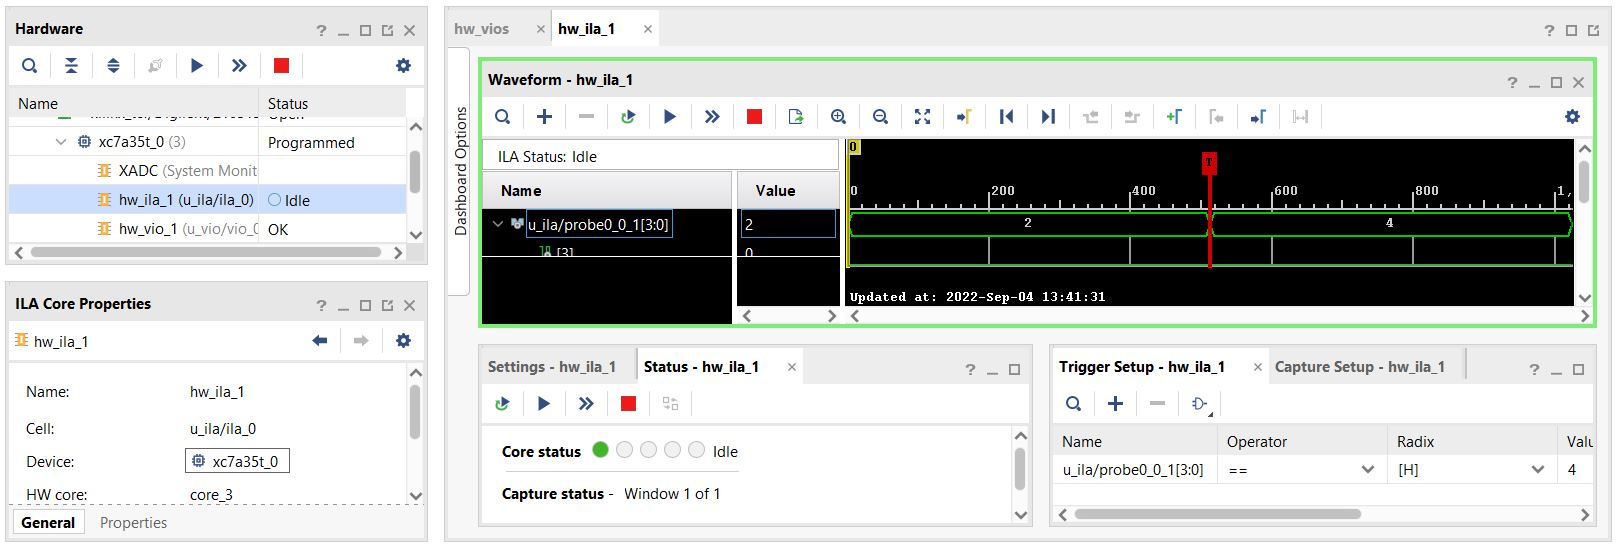
\includegraphics[width=\textwidth]{ila_waveform.jpg}
    \caption{Forma de onda obtenida mediante ILA ante un trigger al leer estado igual a 4 en LEDs}
    \label{fig:ila-waveform}
\end{figure}

\end{document}